
若没有控制结构,CMake语言就不完整!和其他所有东西一样,以命令的形式提供,分为三类:条件块、循环和定义指令。控制结构在脚本中执行,并在项目的构建系统生成过程中执行。

\subsubsubsection{2.5.1\hspace{0.2cm}条件块}

CMake中支持的条件块是不起眼的if()指令。所有条件块必须用endif()关闭,可以有任意数量的elseif()和一个可选的else(),顺序如下:

\begin{lstlisting}[style=styleCMake]
if(<condition>)
	<commands>
elseif(<condition>) # optional block, can be repeated
	<commands>
else() # optional block
	<commands>
endif()
\end{lstlisting}

与许多其他命令式语言一样,if()-endif()块控制将执行哪些指令集:

\begin{itemize}
\item 
若满足if()指令中指定的<condition>表达式,则执行第一部分。

\item 
否则,CMake将在属于该块中满足条件的第一个elseif()指令节中执行命令。

\item 
若没有这样的命令,CMake将检查是否提供了else(),并执行该部分代码中的指令。

\item 
若以上条件都不满足,则在endif()之后继续执行。
\end{itemize}

提供的<condition>表达式根据非常简单的语法求值。

\subsubsubsection{2.5.2\hspace{0.2cm}条件指令的语法}

同样的语法也适用于if()、elseif()和while()指令。

\hspace*{\fill} \\ %插入空行
\noindent
\textbf{逻辑运算符}

if()条件支持NOT、AND和OR逻辑操作符:

\begin{itemize}
\item 
NOT <condition>

\item 
<condition> AND <condition>

\item 
<condition> OR <condition>
\end{itemize}

条件的嵌套也可以通过匹配的括号(())来实现。和所有体面的语言一样,CMake语言尊重求值的顺序,从最里面的括号开始:

\begin{itemize}
\item 
(<condition>) AND (<condition> OR (<condition>))
\end{itemize}

\hspace*{\fill} \\ %插入空行
\noindent
\textbf{字符串和变量的求值}

由于历史原因(因为变量引用(\$\{\})语法并不总是存在),CMake将尝试计算未加引号的参数,就像是变量引用一样。换句话说,在条件中使用普通变量名(例如VAR)等于写入\$\{VAR\}。这里有一个例子:

\begin{lstlisting}[style=styleCMake]
set(VAR1 FALSE)
set(VAR2 "VAR1")
if(${VAR2})
\end{lstlisting}

if()条件在这里的工作方式有点复杂——首先,\$\{VAR2\}求值为VAR1。VAR1是一个可识别的变量,而这个变量的值为FALSE字符串。只有当字符串等于以下任何一个常量时(这些比较不区分大小写),才认为是布尔值true:

\begin{itemize}
\item 
ON, Y, YES或TRUE

\item 
一个非零的数
\end{itemize}

我们得出结论,上例中的条件将计算为false。

这里还有另一个问题——若条件的参数没有加引号,且变量的名称包含一个值,如BAR,那么该如何求值呢?考虑下面的代码示例:

\begin{lstlisting}[style=styleCMake]
set(FOO BAR)
if(FOO)
\end{lstlisting}

根据我们到目前为止所说的,它将是false,因为BAR字符串不满足计算布尔值true值的标准。但情况并非如此,因为CMake在涉及到未加引号的变量引用时会出现例外。与带引号的参数不同,FOO不会通过BAR求值,以生成if("BAR")语句(这将是false)。相反,CMake只会在if(FOO)为false时计算它是以下任何一个常量(这些比较不区分大小写):

\begin{itemize}
\item 
OFF, NO, FALSE, N, IGNORE, NOTFOUND

\item 
以-NOTFOUND结尾的字符串

\item 
一个空字符串

\item 
零
\end{itemize}

因此,未定义的变量将赋值为false:

\begin{lstlisting}[style=styleCMake]
if (FOO)
\end{lstlisting}

但先定义一个变量会改变这种情况,并且计算为true:

\begin{lstlisting}[style=styleCMake]
set(FOO "FOO")
if (FOO)
\end{lstlisting}

\begin{tcolorbox}[colback=blue!5!white,colframe=blue!75!black,title=Note]
若认为不加引号的参数的行为令人困惑,请将变量引用包装在加引号的参数中:if ("\$\{FOO\}")。这将导致在提供的参数传递到if()指令之前进行参数求值,并且行为将与字符串的求值一致。
\end{tcolorbox}

所以,CMake假设用户正在询问是否定义了变量(并且不显式为false)。可以显式检查这个事实(而不用担心值):

\begin{lstlisting}[style=styleCMake]
if(DEFINED <name>)
if(DEFINED CACHE{<name>})
if(DEFINED ENV{<name>})
\end{lstlisting}

\hspace*{\fill} \\ %插入空行
\noindent
\textbf{比较}

以下操作符支持比较操作:

EQUAL,LESS,LESS\_EQUAL,GREATER和GREATER\_EQUAL

可以用来比较数值:

\begin{lstlisting}[style=styleCMake]
if (1 LESS 2)
\end{lstlisting}

\begin{tcolorbox}[colback=blue!5!white,colframe=blue!75!black,title=Note]
CMake文档声明,若其中一个操作数不是数字,则该值将为false。实际实验表明,以数字开头的字符串的比较是正确的:if (20 EQUALS "20 GB")。
\end{tcolorbox}

可以比较[main.[.minor[.patch]]]之后的版本,可以在操作符前添加一个VERSION\_前缀来调整格式:

\begin{lstlisting}[style=styleCMake]
if (1.3.4 VERSION_LESS_EQUAL 1.4)
\end{lstlisting}

省略的组件视为零,非整数版本的组件在该点截断比较字符串。

对于字典字符串比较,需要在操作符前加上STR前缀(注意没有下划线):

\begin{lstlisting}[style=styleCMake]
if ("A" STREQUAL "${B}")
\end{lstlisting}

通常需要比简单的相等比较更高级的机制。

CMake还支持POSIX正则表达式匹配(CMake文档暗示了ERE风格,但没有提到对特定正则表达式字符类的支持).

可以这样使用MATCHES操作符:<variable|string> MATCHES <regex>匹配的组都在CMAKE\_MATCH\_<n>变量中。

\hspace*{\fill} \\ %插入空行
\noindent
\textbf{简单的检查}

已经提到了一个简单的检查,DEFINED。但是还需要其他检查,若满足条件则返回true。

可以检查以下内容:

\begin{itemize}
\item 
若值在列表中:<variable|string> in \_LIST <variable>

\item 
若指令可用:command <command-name>

\item 
若CMake策略存在:POLICY <policy-id>(这将在第3章中介绍)

\item 
若使用add\_test()添加CTest测试:test <test-name>

\item 
若定义了构建目标:target <target-name>
\end{itemize}

我们将在第4章中了解构建目标。现在,只说目标是项目中构建过程的逻辑单元,该项目使用add\_executable()、add\_library()或add\_custom\_target()指令创建,这些指令我们已经使用过了。

\hspace*{\fill} \\ %插入空行
\noindent
\textbf{文件系统检查}

CMake提供了许多处理文件的方法。很少需要直接操作它们,通常会使用高级方法,本书将在附录部分提供与文件相关的命令的简短列表。大多数情况下,只需要以下操作符(行为只对绝对路径有很好的定义):

\begin{itemize}
\item 
EXISTS <path-to-file-or-directory>: 检查文件或目录是否存在

这将解析符号链接(若符号链接的目标存在,则返回true)。

\item 
<file1> IS\_NEWER\_THAN <file2>: 检查哪个文件更新

如果file1比(或等于)file2更新,或者两个文件中有一个不存在,则返回true。

\item 
IS\_DIRECTORY path-to-directory: 检查路径是否为目录

\item 
IS\_SYMLINK file-name: 检查路径是否为符号链接

\item 
IS\_ABSOLUTE path: 检查路径是否为绝对路径
\end{itemize}

\subsubsubsection{2.5.3\hspace{0.2cm}循环}

CMake中的循环相当简单——可以使用while()或foreach()重复执行同一组命令。这两个命令都支持循环控制机制:

\begin{itemize}
\item 
break()循环停止剩余块的执行,并从封闭循环中断开。

\item 
continue()循环停止当前迭代的执行,并开启下一个迭代。
\end{itemize}

\hspace*{\fill} \\ %插入空行
\noindent
\textbf{While}

循环块用while()指令创建,用endwhile()关闭。只要while()中提供的<condition>表达式为true,其后续的指令都会执行。条件语句的语法与if()指令相同:

\begin{lstlisting}[style=styleCMake]
while(<condition>)
	<commands>
endwhile()
\end{lstlisting}

通过一些额外的变量——while循环可以替换for循环。实际上,使用foreach()循环要容易得多。

\hspace*{\fill} \\ %插入空行
\noindent
\textbf{Foreach}

foreach块有几个变体,为每个值执行附带的指令,它有打开和关闭指令:foreach()和endforeach()。

foreach()最简单的形式是为了提供C++风格的for循环:

\begin{lstlisting}[style=styleCMake]
foreach(<loop_var> RANGE <max>)
	<commands>
endforeach()
\end{lstlisting}

CMake将从0迭代到<max>(包括)。若需要更多的控制,可以使用第二个变量,提供<min>、<max>和<step>(可选)。所有参数必须是非负整数。同时,<min>必须小于<max>:

\begin{lstlisting}[style=styleCMake]
foreach(<loop_var> RANGE <min> <max> [<step>])
\end{lstlisting}

然而,foreach()在处理列表时展示了它的真面目:

\begin{lstlisting}[style=styleCMake]
foreach(<loop_variable> IN [LISTS <lists>] [ITEMS <items>])
\end{lstlisting}

CMake将从所有提供的<lists>列表变量中获取元素,然后是所有显式声明的<items>值,并将它们存储在<loop\_variable>中,对每个项逐个执行<commands>。可以选择只提供列表,只提供值,或者两者都提供:

\begin{lstlisting}[style=styleCMake]
# chapter02/06-loops/foreach.cmake

set(MY_LIST 1 2 3)
foreach(VAR IN LISTS MY_LIST ITEMS e f)
	message(${VAR})
endforeach()
\end{lstlisting}

上述代码将打印以下内容:

\begin{tcblisting}{commandshell={}}
1 
2 
3 
e 
f
\end{tcblisting}

或者,使用一个简短的版本(跳过IN关键字)来获得相同的结果:

\begin{lstlisting}[style=styleCMake]
foreach(VAR 1 2 3 e f)
\end{lstlisting}

从3.17版本开始,foreach()已经学会了如何压缩列表(ZIP\_LISTS):

\begin{lstlisting}[style=styleCMake]
foreach(<loop_var>... IN ZIP_LISTS <lists>)
\end{lstlisting}

压缩列表可以遍历多个列表并处理具有相同索引的各自项:

\begin{lstlisting}[style=styleCMake]
# chapter02/06-loops/foreach.cmake

set(L1 "one;two;three;four")
set(L2 "1;2;3;4;5")
foreach(num IN ZIP_LISTS L1 L2)
	message("num_0=${num_0}, num_1=${num_1}")
endforeach()
\end{lstlisting}

CMake将为每个提供的列表创建一个num\_<N>变量,用每个列表中的项填充该变量。可以传递多个<loop\_var>变量名(每个列表一个),每个列表将使用单独的变量来存储:

\begin{lstlisting}[style=styleCMake]
foreach(word num IN ZIP_LISTS L1 L2)
	message("word=${word}, num=${num}")
\end{lstlisting}

若列表之间的项数不同,CMake将不会为较短的列表定义变量。

以上就是关于循环的所有内容。

\subsubsubsection{2.5.4\hspace{0.2cm}定义指令}

有两种方法可以定义自己的命令:可以使用macro()或function()。要解释这两个指令间的区别,最简单的方法是将它们与C风格的宏和实际的C++函数进行比较:

\begin{itemize}
\item 
macro()的工作方式更像是查找和替换指令,而不是像function()这样的实际子例程调用。与函数相反,宏不会在调用堆栈上创建单独的条目。所以宏中调用return()将比在函数中返回调用语句的级别高一级(若已经在顶层作用域中,可能会终止执行)。

\item 
function()为本地变量创建一个单独的作用域,这与macro()命令不同,后者在调用者的变量作用域中工作。这可能会导致令人困惑的结果。让我们在下一节中讨论其中细节。
\end{itemize}

这两个方法都接受可以在命令块中命名和引用的参数。此外,CMake允许通过以下引用访问命令调用中传递的参数:

\begin{itemize}
\item 
\$\{ARGC\}: 参数的数量

\item 
\$\{ARGV\}: 所有参数的列表

\item 
\$\{ARG0\}, \$\{ARG1\}, \$\{ARG2\}: 特定索引处的实参值

\item 
\$\{ARGN\}: 最后一个预期参数之后,由调用者传递的匿名参数列表
\end{itemize}

使用ARGC边界外的索引访问数值参数会产生未定义行为。

若确定需要定义一个带有命名参数的指令,则每次调用都必须传递所有这些参数,否则将无效。

\hspace*{\fill} \\ %插入空行
\noindent
\textbf{宏}

定义宏类似于任何其他块:

\begin{lstlisting}[style=styleCMake]
macro(<name> [<argument>…])
	<commands>
endmacro()
\end{lstlisting}

此声明之后,可以通过调用宏的名称来执行宏(函数调用不区分大小写)。

下面的例子强调了与宏中变量作用域相关的问题:

\begin{lstlisting}[style=styleCMake]
# chapter02/08-definitions/macro.cmake

macro(MyMacro myVar)
	set(myVar "new value")
	message("argument: ${myVar}")
endmacro()

set(myVar "first value")
message("myVar is now: ${myVar}")
MyMacro("called value")
message("myVar is now: ${myVar}")
\end{lstlisting}

下面是这个脚本的输出:

\begin{tcblisting}{commandshell={}}
$ cmake -P chapter02/08-definitions/macro.cmake
myVar is now: first value
argument: called value
myVar is now: new value
\end{tcblisting}

发生了什么事?尽管显式地将myVar设置为新值,但并不影响message("argument:\$\{myVar\}")!这是因为传递给宏的参数没有视为真正的变量,而是作为常量查找并替换指令。

另一方面,全局作用域中的myVar变量从第一个值更改为新值。这种行为称为副作用,是一种糟糕的实践,因为在不了解宏的情况下,很难判断哪些变量可能会受到这种宏的影响。

建议尽可能使用函数,可以避免许多令人头疼的事情。

\hspace*{\fill} \\ %插入空行
\noindent
\textbf{函数}

将指令声明为函数,可以使用以下语法:

\begin{lstlisting}[style=styleCMake]
function(<name> [<argument>…])
	<commands>
endfunction()
\end{lstlisting}

函数需要一个名称,并可选地接受预期参数的名称列表。

若函数调用传递的参数多于声明的参数,多余的参数将解释为匿名参数并存储在ARGN变量中。

如前所述,函数开放自己的作用域。可以调用set(),提供函数的一个命名参数,任何更改都将是函数的局部更改(除非指定了PARENT\_SCOPE)。

函数遵循调用堆栈的规则,允许使用return()返回调用作用域。

CMake为每个函数设置以下变量(从3.17版本开始提供):

\begin{itemize}
\item 
CMAKE\_CURRENT\_FUNCTION

\item 
CMAKE\_CURRENT\_FUNCTION\_LIST\_DIR

\item 
CMAKE\_CURRENT\_FUNCTION\_LIST\_FILE

\item 
CMAKE\_CURRENT\_FUNCTION\_LIST\_LINE
\end{itemize}

来看看这些函数变量在实践中的情况:

\begin{lstlisting}[style=styleCMake]
# chapter02/08-definitions/function.cmake

function(MyFunction FirstArg)
	message("Function: ${CMAKE_CURRENT_FUNCTION}")
	message("File: ${CMAKE_CURRENT_FUNCTION_LIST_FILE}")
	message("FirstArg: ${FirstArg}")
	set(FirstArg "new value")
	message("FirstArg again: ${FirstArg}")
	message("ARGV0: ${ARGV0} ARGV1: ${ARGV1} ARGC: ${ARGC}")
endfunction()

set(FirstArg "first value")
MyFunction("Value1" "Value2")
message("FirstArg in global scope: ${FirstArg}")
\end{lstlisting}

输出如下:

\begin{tcblisting}{commandshell={}}
Function: MyFunction
File: /root/examples/chapter02/08-definitions/function.cmake
FirstArg: Value1
FirstArg again: new value
ARGV0: Value1 ARGV1: Value2 ARGC: 2
FirstArg in global scope: first value
\end{tcblisting}

函数的一般语法和概念非常类似于宏,但这一次是有效的。

\hspace*{\fill} \\ %插入空行
\noindent
\textbf{CMake中的过程范式}

想象一下,我们用C++编写程序的相同方式编写一些CMake代码。将创建一个CMakeLists.txt列表文件,将调用三个定义的指令,这些指令可能调用它们自己定义的指令:

\begin{center}
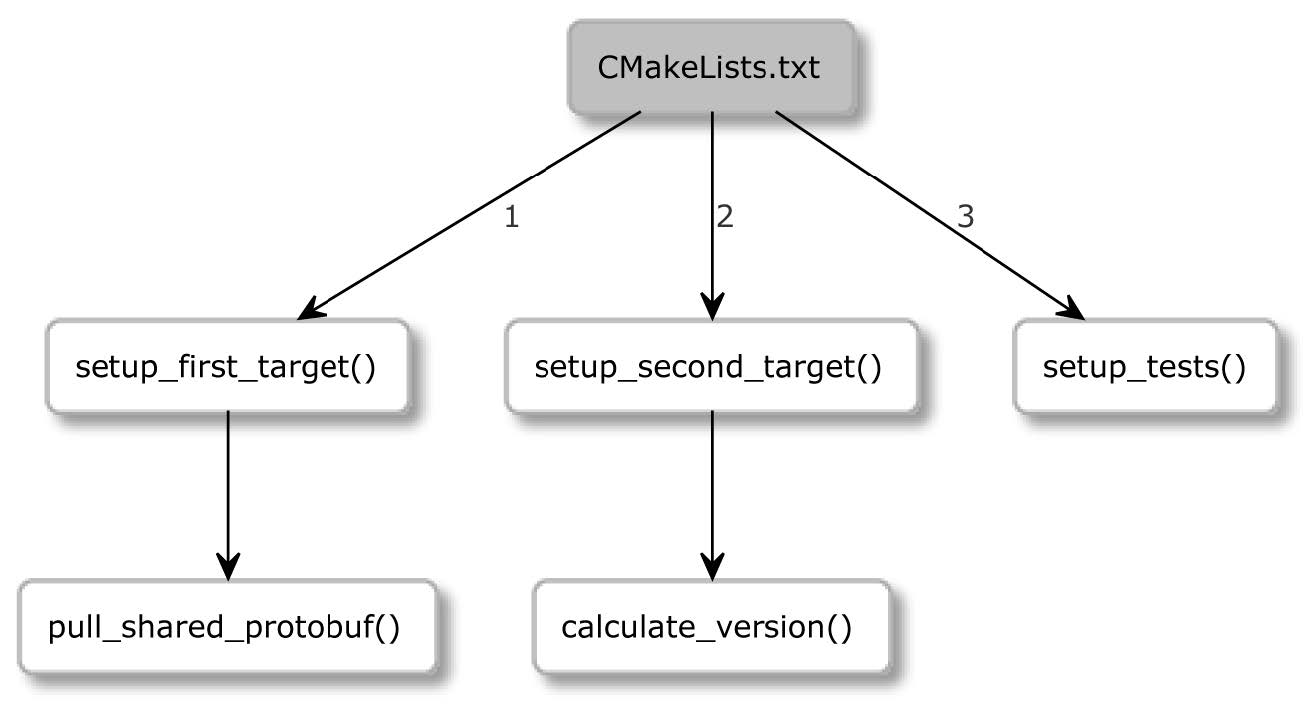
\includegraphics[width=0.8\textwidth]{content/1/chapter2/images/3.jpg}\\
图2.3 调用图
\end{center}

CMake中,用这种过程风格编写代码有点麻烦——需要提前提供计划使用的命令定义:

\begin{lstlisting}[style=styleCMake]
cmake_minimum_required(...)
project(Procedural)
function(pull_shared_protobuf)
function(setup_first_target)
function(calculate_version)
function(setup_second_target)
function(setup_tests)

setup_first_target()
setup_second_target()
setup_tests()
\end{lstlisting}

真是恶梦一场!这段代码非常难以阅读,因为最微小的细节都在文件的顶部。一段结构正确的代码在第一个子例程中列出最通用的步骤,之后提供稍微详细一些的子例程,并将最详细的步骤推到文件的最后。

对于这个问题有一些解决方案:将命令定义移动到其他文件和跨目录分区作用域(作用域目录将在第3章中详细解释)。但也有一个简单而优雅的解决方案:在文件的顶部声明一个入口点宏,并在文件的最后调用它:

\begin{lstlisting}[style=styleCMake]
macro(main)
function(...) # key steps
function(...) # details
function(...) # fine details
main()
\end{lstlisting}

通过这种方法,代码的编写范围逐渐缩小,因为直到最后我们才真正调用main()宏,CMake不会抱怨未定义命令的执行!

最后一个问题仍然存在——为什么在推荐的函数上使用宏?可以无限制地访问全局变量,因为没有向main()传递参数,所以通常不需要担心这里的警告。

可以在本书的GitHub存储库中的chapter-02/09-procedural/CMakeLists.txt列表文件中找到这个简单例子。

\hspace*{\fill} \\ %插入空行
\noindent
\textbf{关于命名约定}

软件开发中,命名非常困难,但维护易于阅读和理解的解决方案非常重要。当涉及到CMake脚本和项目时,应该遵循干净代码方法的规则,就像对待软件开发解决方案一样:

\begin{itemize}
\item 
遵循一致的命名风格(snake\_case是CMake社区接受的标准)。

\item 
使用简短但有意义的名称(例如,避免func()、f()等)。

\item 
避免双关语和难懂的命名。

\item 
使用容易发音、容易搜索的名字,不需要人为映射。
\end{itemize}

现在已经知道了如何使用正确的语法正确地调用指令,让我们从使用指令开始研究。
















